\documentclass[12pt,a4paper]{article}

\usepackage{geometry}
 \geometry{
 a4paper,
 total={170mm,257mm},
 left=20mm,
 top=20mm,
 }
 \usepackage{listings}
 \usepackage{color}

\definecolor{mygreen}{rgb}{0,0.6,0}
\definecolor{mygray}{rgb}{0.5,0.5,0.5}
\definecolor{mymauve}{rgb}{0.58,0,0.82}

\lstset{ %
  backgroundcolor=\color{white},   % choose the background color; you must add \usepackage{color} or \usepackage{xcolor}; should come as last argument
  basicstyle=\ttfamily\footnotesize,        % the size of the fonts that are used for the code
  breakatwhitespace=false,         % sets if automatic breaks should only happen at whitespace
  breaklines=true,                 % sets automatic line breaking
  captionpos=b,                    % sets the caption-position to bottom
  commentstyle=\color{mygreen},    % comment style
  deletekeywords={...},            % if you want to delete keywords from the given language
  escapeinside={\%*}{*)},          % if you want to add LaTeX within your code
  extendedchars=true,              % lets you use non-ASCII characters; for 8-bits encodings only, does not work with UTF-8
  %frame=single,	                   % adds a frame around the code
  keepspaces=true,                 % keeps spaces in text, useful for keeping indentation of code (possibly needs columns=flexible)
  keywordstyle=\color{blue},       % keyword style
  language=Python,                 % the language of the code
  morekeywords={*,...},           % if you want to add more keywords to the set
  numbers=left,                    % where to put the line-numbers; possible values are (none, left, right)
  numbersep=5pt,                   % how far the line-numbers are from the code
  numberstyle=\tiny\color{mygray}, % the style that is used for the line-numbers
  rulecolor=\color{black},         % if not set, the frame-color may be changed on line-breaks within not-black text (e.g. comments (green here))
  showspaces=false,                % show spaces everywhere adding particular underscores; it overrides 'showstringspaces'
  showstringspaces=false,          % underline spaces within strings only
  showtabs=false,                  % show tabs within strings adding particular underscores
  stepnumber=2,                    % the step between two line-numbers. If it's 1, each line will be numbered
  stringstyle=\color{mymauve},     % string literal style
  tabsize=2,	                   % sets default tabsize to 2 spaces
  title=\lstname                   % show the filename of files included with \lstinputlisting; also try caption instead of title
}

\usepackage[english]{babel}
\usepackage[utf8]{inputenc}
\usepackage{amsmath}
\usepackage{amsfonts}
\usepackage{bm}
\usepackage{graphicx,caption,subcaption,float}
%\usepackage{fullpage}

\bibliographystyle{plain}

\title{\Huge  Time Series Analysis in Python: User Manual}

\author{Wenyan Gong, Zongxi Li, Cong Ma
\\Qingcan Wang, Zhuoran Yang, Hao Zhang}

\date{\today}

\begin{document}
\maketitle

\section{Introduction}
Time series analysis comprises methods for analyzing time series data in order to extract meaningful statistics and other characteristics of the data. It is widely used in signal processing, pattern recognition, mathematical finance, weather forecasting, earthquake prediction, control engineering, and largely in any domain of applied science and engineering which involves temporal measurements.

In this project, we will play a game with time series in finance. It has gained its popularity in Wall Street recently, since it is fundamental to most promising quantitative investment strategies. We develop a system that can predict future prices of stocks using various kinds of methods for time series analysis. 

This manual is a brief introduction of the functionality of our package. In specific,  we illustrate  how to use the provided functions to fit the model, predict the stock price, trade, cluster etc. Introduction of the main source files and key functions is also included.

We  utilize standard packages from python including \texttt{numpy}, \texttt{scipy}, and \texttt{matplotlib}. The integration of \texttt{C} code  and \texttt{Python} code is based on the \texttt{Cython} package.

\section{Program Structure}
The high-level program structure is shown in Figure \ref{fig:structure}. The division of work is pretty even, and there are some minor work that are too trivial to mention extensively here. 
\begin{figure}[htp]
        \centering
     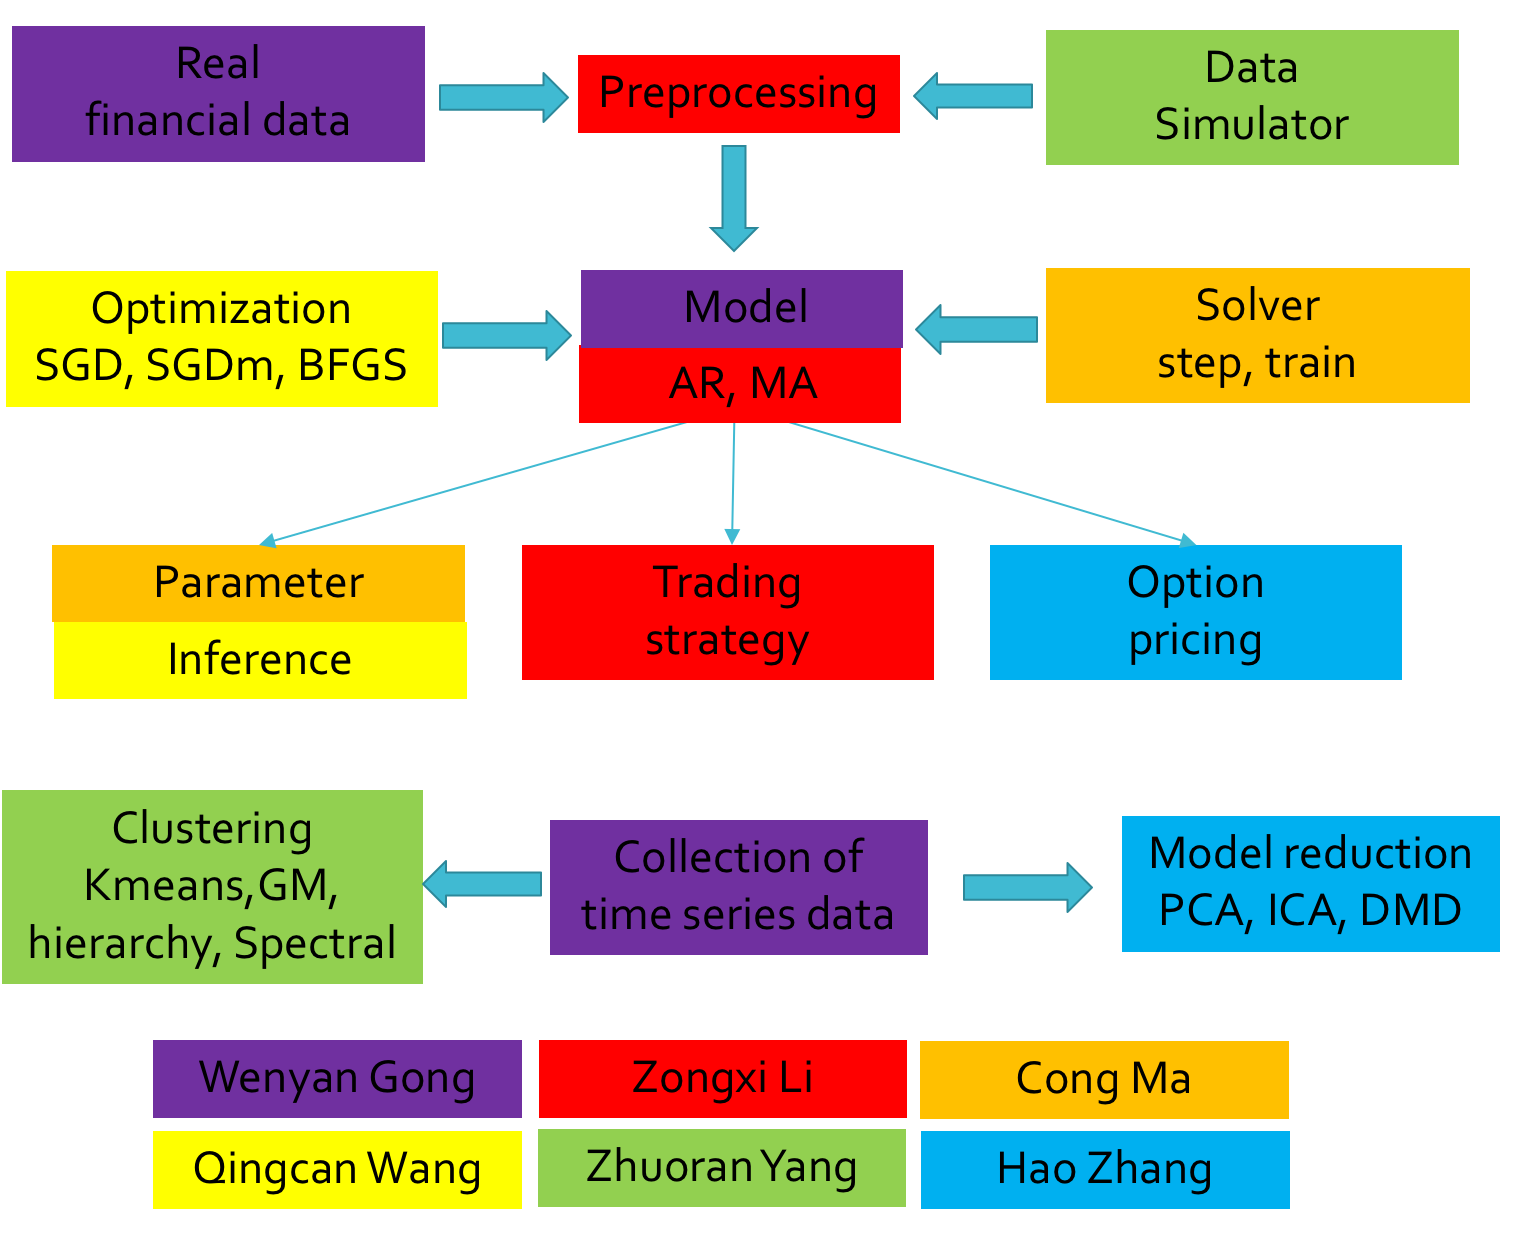
\includegraphics[width=.8\linewidth]{./Figure/structure.png}
\caption{Program structure and division of work}
\label{fig:structure}
\end{figure}
Overall, the program consists of two parts. The first part deals with a single time series, and exploits the time correlation within the time series. There is data preprocessing module that takes the raw data and get the right data format for later analysis. Optimization, model, and solver are used all together to fit the models using maximum likelihood estimation. Finally, there is a post processing module that makes use of the information from model. The post processing module includes parameter inference, trading strategy, and option pricing. The second part deals with a collection of time series of data, basically it exploits the correlation between different time series. In this way, we can gain more insights into the financial market. While these insights are impossible to obtain from a single time series.

\section{Functionality}
To start with, we will give an description of the source files.
\begin{itemize}
\item \texttt{basemodel.py}: Provided the basemodel of time series.
\item \texttt{cluster.py}:  Provided the \texttt{Cluster} class for clustering. It includes four clustering methods: k-means, hierarchy clustering, Gaussian mixture modeling, and spectral clustering.
\item \texttt{Data\_prossessor.py}:  Provided the transforming function between stock price and return, the function getting the maximum drawdown and the function returning the indicator of peak and trough.

\item \texttt{Gradient\_check.py}: Provided the function for deriving numerical gradient.

\item \texttt{Inference.py}: Provided functions for computing the auto-covariance of \texttt{AR} model and testing significance of parameters.

\item \texttt{Model.py}: Provided model class \texttt{AR} and \texttt{MA}, including functions for computing the log-likelihood and gradient given the data and an \texttt{AR} or \texttt{MA} model and the function for future price prediction.

\item \texttt{Optim.py}: Provided several optimization methods: stochastic gradient descent, stochastic gradient descent with momentum update and Broyden–Fletcher–Goldfarb–Shanno algorithm

\item \texttt{Option\_pricing.py}: Provided functions for option pricing.

\item \texttt{Reduction.py}: Provided functions for dimensional reduction for data visualization.

\item \texttt{Solver.py}: Provided functions for model fitting using maximum likelihood estimation given the data and the specified model.

\item \texttt{Trading.py}: Provided functions for deciding the transaction time point based on future price prediction and computing profit over the time.

\item \texttt{Ts\_gen.pyx} \& \texttt{c\_ts\_gen.c}: Provided functions to generate simulation data.

\end{itemize}

\subsection{Data Preparation and Preprocessing}
%!TEX root = ../../manual.tex
We provide both a real dataset and methods to generate simulated data from various time series models.  For data simulation,  we provide functions that samples from the \texttt{AR(p), MA(q), ARMA (p,q), GARCH(p,q)} models, which is written in \texttt{C} code. See \texttt{c\_ts\_gen.c} for the source code. To integrate \texttt{C} code into \texttt{Python}, we write a \texttt{Cython} wrapper \texttt{ts\_gen.pyx}, which generates a \texttt{Python} module named \texttt{ts\_gen}. This module consists of five functions.  The inputs of these functions all consist  of four  elements: 
\begin{enumerate}
\item  \texttt{param}: a \texttt{numpy Nd array} or a few \texttt{float} numbers -- the model parameters.
\item \texttt{time}:  an  \texttt{integer} -- the total time of the time series.
\item  \texttt{num}: an  \texttt{integer} -- number of independent sample paths, 
\item \texttt{burnin}: an  \texttt{integer} -- the length of burnin period. This parameter has default value $2000$. 
\end{enumerate} 
These functions all output a \texttt{numpy Nd array} with dimension $( \texttt{num} \times \texttt{time})$ which stores  \texttt{num} independent paths of the time series data until $T = \texttt{time}$. Functions that generate simulated data are listed as follows. 
 
  \begin{lstlisting}[language=Python]
-ar1_gen(double rho, double sigma, int time, int num, int burnin)
-ma1_gen( double rho, double constant,  int time,  int num,  int burnin 
-arch1_gen(double a0, double a1, int time, int num, int burnin)
-garch11_gen(double a, double b, double c, const int time, const int num, const int burnin 
-garch11_gen(double a, double b, double c, const int time, const int num, const int burnin )
-arma_gen( np.ndarray[double, ndim=1, mode="c"] ar, int p, np.ndarray[double, ndim=1, mode="c"]  ma, const int q, const double sigma,
const int time, const int num, const int burnin)
\end{lstlisting}
For an example of usage, see the following example. 
   \begin{lstlisting}[language=Python]
from tsap.ts_gen import arma1_gen
import numpy as np
Y = ar1_gen(0.5, sigma = 1.0, time = 200, num = 10, burnin = 2000)
print(Y.shape)
\end{lstlisting}
The output, as expected, is
   \begin{lstlisting}[language=Python]
>>(10, 200)
\end{lstlisting}

\subsection{Model}
The model related functions are written in \texttt{model.py}, which contains two model classes: AR and MA. They are used to fit an AR or MA model by given parameters, to compute the log-likelihood and gradients given an AR or MA model and the data and to give predictions. The functions are introduced below.
Firstly, you can fit an AR or MA model by given parameters. The inputs are as follows: 
\begin{enumerate}
\item \texttt{lag}: the lag parameter for the fitted model, a number;
\item \texttt{phi}: the coefficients for the fitted model, a \texttt{numpy} array whose dimension is the \texttt{lag} given above;
\item \texttt{sigma}: the variance of noise for the fitted model, a number;
\item \texttt{intercept}: the intercept of noise for the fitted model, a number.
\end{enumerate}
The output is a model object.
To fit the model, we can run
\begin{lstlisting}[language=Python]
AR_model = AR(lag=3, phi=np.array([[1],[1],[1]]), sigma=1, intercept=0.1)
MA_model = MA(lag=3, phi=np.array([[1],[1],[1]]), sigma=1, intercept=0.1)
\end{lstlisting}
Secondly, you can compute the log-likelihood and gradients given an AR or MA model and the data. The input is as follows:
\begin{enumerate}
\item \texttt{data}: One or several time series. The input data should be a 2-dimensional array. Each row of data represents a time series over the time, e.g. the stock return over the year of a single stock. The number of rows should be the number of time series.
\end{enumerate}
The output is a number for the computed loglikelihood and a tuple for the computed gradients. This function is public but mostly it serve for the \texttt{Solver} class. 
To compute the log-likelihood and the gradients, we can run 
\begin{lstlisting}[language=Python]
AR_llh, AR_grads= AR_model.loss(data)
MA_llh, MA_grads= MA_model.loss(data)
\end{lstlisting}
Finally, you can make prediction based on a fitted model. The input is as follows:
\begin{enumerate}
\item \texttt{data}: the time series before the first prediction. The number of columns (the length of the time series) should exceed the given lag for a reasonable prediction;
\item \texttt{nstep}: the number of predictions.
\end{enumerate}
To make predictions, we can run
\begin{lstlisting}[language=Python]
AR_future=AR_model.predict(data,nstep=5)
MA_future=MA_model.predict(data,nstep=5)
\end{lstlisting}





\subsection{Optimization}
%!TEX root = ../../manual.tex

The optimization part \texttt{optim.py} implements various optimization update
rules: stochastic gradient descent (\texttt{sgd}), stochastic gradient descent
with momentum update (\texttt{sgd\_momentum}) and
Broyden–Fletcher–Goldfarb–Shanno algorithm (\texttt{bfgs}). 

Each update rule accepts current iteration point and the gradient of the object
function and produces the next iteration point. Each update rule has the same
interface:
\begin{lstlisting}[language=Python]
def update(x, dx, config=None):
\end{lstlisting}
The inputs are as follows:
\begin{enumerate}
  \item \texttt{x}:
    A \texttt{numpy} array giving the current iteration point.
  \item \texttt{dx}:
    A \texttt{numpy} array of the same shape as \texttt{x} giving the gradient
    of the object function with respect to \texttt{x}.
  \item \texttt{config}:
    A dictionary containing hyper-parameter values such as learning rate,
    momentum, etc. If the update rule requires caching values over many
    iterations, then config will also hold these cached values.
\end{enumerate}
The outputs are as follows:
\begin{enumerate}
  \item \texttt{next\_x}:
    The next point after the update.
  \item \texttt{config}:
    The config dictionary to be passed to the next iteration of the update rule.
\end{enumerate}

The update rules are called in \texttt{Solver} class like this:
\begin{lstlisting}[language=Python]
objfcn, grads = self.model.objfcn(self.X)
for p, x in self.model.params.iteritems():
    dx = grads[p]
    config = self.optim_configs[p]
    next_x, next_config = self.update_rule(x, dx, config)
    self.model.params[p] = next_x
    self.optim_configs[p] = next_config
\end{lstlisting}



\subsection{Solver}
%!TEX root = ../../report.tex
We develop a solver class, which serves as a bridge between the model class and the optimization methods. Specifically, given the loss function and the gradient functions specified by the model and the optimization methods, the solver uses this method to minimize the loss until it converges. 
\subsection{Inference}
%!TEX root = ../../manual.tex

The methods that perform statistical inference is written in \texttt{inference.py}, which consists of five functions, i.e., \texttt{acovf}, \texttt{acf}, \texttt{BL\_stat}, \texttt{yule\_walker}, and  \texttt{ar\_select}.  In the following, we give a detailed introduction of the usages of these functions.
Firstly, \texttt{acovf} and  \texttt{acf} returns the auto-covariance and auto-correlations of one path of time series. The input include 
\begin{enumerate}
\item \texttt{x}: an one dimensional \texttt{numpy} array.
\item \texttt{demean}: a boolean variable that tells whether to subtract the mean.
\item  \texttt{nlags}: maximum order of lags in autocorrelation.
\item  \texttt{fft}: boolean, whether use fast Fourier transform.
\end{enumerate}
The output is an array of auto-covariance or auto-correlation. 
To use these function, we can run 
\begin{lstlisting}[language=Python]
auto_cov = acovf(x, demean=True, fft=False) 
auto_cor = acf(x, nlags = 40, demean=True, fft=False)
\end{lstlisting}
Secondly, \texttt{BL\_stat} performs Box-Ljung test that tests if the time series data are correlated.     The input are \texttt{acf\_array},  which is  an array of auto-correlation coefficients (ACF), \texttt{order}, which is the maximum order of ACF used,   and \texttt{nobs}, which is the time length that is used to compute the ACF. The outputs are the test statistic, a float number , the $p$-value, also a float number, and the test result, which  a boolean. To use this function, an example is 
\begin{lstlisting}[language=Python]
test_stat, pval, test_result = BL_stat(acf_array, order, nobs):
\end{lstlisting}
Finally,  \texttt{yule\_walker}  and  \texttt{ar\_select} are specified for the \texttt{AR(p)} model.   In specific, \texttt{ar\_select} takes an array of time series   as input and outputs the estimated order of the autoregresive model. Whereas  \texttt{yule\_walker} takes the time series and the order as input and outputs the estimated parameters using Yule Walker method. The usage will be clear from the following example.
\begin{lstlisting}[language=Python]
import tsap.inference as inference
from tsap.ts_gen import ar1_gen

ts = ar1_gen(0.3, sigma = 1.0, time = 500, num = 1, burnin = 2000)
order_est = inference.ar_select(ts)
print("The estimated order of AR model is "+ str(order_est))
rho, sigma = inference.yule_walker(ts, order = 1)
print("The estimated model parameter is "+ str(rho))
\end{lstlisting}
The output is 
\begin{lstlisting}[language=Python]
>>The estimated order of AR model is 2
>>The estimated model parameter is [ 0.2973149]
\end{lstlisting}

\subsection{Trading Strategy}
%!TEX root = ../../manual.tex

The functions for trading is written in \texttt{trading.py}, which consists of four functions, i.e., \texttt{signal\_generation}, \texttt{profit\_loss}, \texttt{trade}, and \texttt{rolltrade}.  In the following, we give a detailed introduction of the usage of these functions.

Firstly, \texttt{signal\_generation} returns the trading signal, like what time to buy and what time to sell. The input includes
\begin{enumerate}
\item \texttt{X}: a one dimensional \texttt{numpy} array, which is the price series.
\item \texttt{window}: a positive integer that specifies the largest length of one trade. If \texttt{window}=5, that means there's at most one trade activity within 5 days. The default number is 2.
\end{enumerate}
The output is a one dimensional numpy array, whose elements are 1 (buying signal), -1 (selling signal), 0 (no signal).
To use these function, we can run 
\begin{lstlisting}[language=Python]
import trading 
signal = trading.signal_generation(X, window = 5) 
\end{lstlisting}

Secondly, \texttt{signal\_generation} returns the profit based on given trading signals. The input includes
\begin{enumerate}
	\item \texttt{X}: a one dimensional \texttt{numpy} array, which is the price series.
	\item \texttt{signal}: a one dimensional \texttt{numpy} array that contains trading signals. Usually, it takes the output of \texttt{signal\_generation}.
	\item \texttt{money}: a positive float number, which is the initial wealth. The default number is 1.
\end{enumerate}
The output is a one dimensional numpy array, which is the time series of profit at different time points.
To use these function, we can run 
\begin{lstlisting}[language=Python]
import trading 
signal = trading.signal_generation(X, window = 5) 
profit = trading.profit_loss(Y, signal, money = 100) 
\end{lstlisting}

Next, \texttt{trade} returns the profit in certain time period. Specifically, given a fitted model, it uses this model to forecast future returns based on historical returns, which are obtained by transfering historical prices 
to historical returns. After that, it again transfers the returns to prices and then generates trading signal 
based on predicted prices. At last it calculates the profit based on the real price series and the trading signals. The input includes
\begin{enumerate}
	\item \texttt{X}: a one dimensional \texttt{numpy} array, which is historical price.
	\item \texttt{Y}: a one dimensional \texttt{numpy} array, which is future prices.
	\item \texttt{M}: a class from \texttt{model.py}, which is a fitted model.
	\item \texttt{nstep}: an positive integer, which specifies how many steps to predict.
    \item \texttt{window}: an positive integer that specifies the largest length of one trade. If \texttt{window}=5, that means there's at most one trade activity within 5 days. 
	\item \texttt{money}: a positive float number, which is the initial wealth. The default number is 1.0.
\end{enumerate}
The output is a one dimensional numpy array, which is the time series of profit at different time points.
To use these function, we can run 
\begin{lstlisting}[language=Python]
import trading
import model
AR_model = model.AR(lag=3, phi=np.array([[1],[1],[1]]), sigma=1, intercept=0.1)
profit = trading.trade(X, Y, M = AR_model, nstep = 10, window = 5, money = 100) 
\end{lstlisting}


Lastly, \texttt{rolltrade} returns the profit, trading signal, and the predicted prices by rolling trading in the whole time period, which is an extension of \texttt{trade}. It will repeat the following procedure until the data is used up. Specifically, given a fitted model, it uses this model to forecast future returns based on historical returns, which are obtained by transfering historical prices 
to historical returns. After that, it again transfers the returns to prices and then generates trading signal 
based on predicted prices. At last it calculates the profit based on the real price series and the trading signals. The input includes
\begin{enumerate}
	\item \texttt{X}: a one dimensional \texttt{numpy} array, which is historical price.
	\item \texttt{M}: a class from \texttt{model.py}, which is a fitted model.
	\item \texttt{l}: an integer number, which specifies how many data points are used to train for each trading.
	\item \texttt{nstep}: an positive integer, which specifies how many steps to predict.
	\item \texttt{window}: an positive integer that specifies the largest length of one trade. If \texttt{window}=5, that means there's at most one trade activity within 5 days. 
	\item \texttt{money}: a positive float number, which is the initial wealth. The default number is 1.0.
\end{enumerate}
The output is three one-dimensional numpy array, which are the time series of profit, trading signal, and the predicted prices at different time points.
To use these function, we can run 
\begin{lstlisting}[language=Python]
# import library
import trading 
import model
import numpy as np
import data_processor as dp

# read data and do the preprocessing
data = np.loadtxt("../data/GOOG.csv", delimiter=',')
X = np.array([data[0:100]])
Y = dp.get_return(X)

# initialize the model
lag = 5
sigma = 1.0
intercept = 0.1
phi = np.array([[ 0.04560256],[ 0.0535601 ],[-0.78190871],[ 1.30062633],[ 0.46616754]])
AR_model = AR(lag=lag, phi=phi, sigma=sigma, intercept=intercept)

# solve the model
_, grads = AR_model.loss(Y)
solver = Solver(AR_model, Y, update_rule='sgd_momentum', optim_config={'learning_rate': 1e-6,}, num_epochs=10000, batch_size=1,print_every=10)
solver.train()

# get the trading profit, signal and predicted price
profit, signal, out_pred_price = trading.rolltrade(X, M = AR_model, l = 100, nstep = 20, window = 5, money = 100) 
\end{lstlisting}

\subsection{Option Pricing}
%!TEX root = ../../manual.tex

The class \texttt{OptionPricing} calculates the call option price of an underlying
stock based on the Black-Scholes model.

The following parameters are needed to construct an instance of the
\texttt{OptionPricing} class:
\begin{enumerate}
  \item \texttt{sigma}:
    the volatility of the underlying stock price, which is the standard
    deviation of the stock's returns.
  \item \texttt{K}:
    the strike price of the option.
  \item \texttt{T}:
    the expiry time of the option.
  \item \texttt{r}:
    the risk-free interest rate.
  \item \texttt{Smax}:
    the maximum stock price we want to consider.
\end{enumerate}

The method \texttt{solve\_black\_scholes} calculates the option pricing of an
instance, given the grid size of price and time (\texttt{nS} and \texttt{nt}) as
input parameters. The option price as an function of stock price and time will
be stored in the instance.

After running \texttt{solve\_black\_scholes}, we can use 
\texttt{get\_option\_price} method to get the option price of given underlying
stock price \texttt{S} and time \texttt{t}.

Following is a usage example of the \texttt{OptionPricing} class:
\begin{lstlisting}[language=Python]
goog = np.genfromtxt("../data/GOOG.csv", delimiter=",")
sigma = np.std((goog[1:] - goog[:-1]) / goog[:-1])

option_price = OptionPricing(sigma=sigma, T=90, K=800, r=0.005, Smax=1200)
option_price.solve_black_scholes(nS=100, nt=300)
print(option_price.get_option_price(S=810, t=30))
\end{lstlisting}


\subsection{Clustering}
%!TEX root = ../../manual.tex
We also provide realizations of four clustering methods: K-means, spectral clustering, hierarchical clustering, and Gaussian mixture modeling. These methods are organized by  the \texttt{Cluster} class, which is initialized by an input data matrix of dimension $(\texttt{nsample}\times \texttt{nfeature})$ where \texttt{nsample} is the number of data points and \texttt{nfeature} is the number of features.  An object in the class consists of three attributes:\texttt{\_X}, which stores the data matrix,  \texttt{\_nsample}, and  \texttt{\_nfeature}. All clustering functions in this class is  has the form 
\begin{lstlisting}[language=Python]
centroid, labels, clusters =Clustering_method(self, nClusters, maxIter)
\end{lstlisting}
Here \texttt{Clustering\_method} is one of \texttt{Kmeans}, \texttt{H\_clustering},  \texttt{Spectral}, and \texttt{Gaussian\_mixture}. In addition, \texttt{nClusters} is the number of clusters and \texttt{maxIter} is the maximum number of iterations, which has default value $300$. The output consists of three items.  \texttt{centroid}, a $\texttt{nClusters} \times \texttt{\_nfeatures} $ matrix storing the centers of clusters; \texttt{labels} is the predicted labels; \texttt{clusters} stores the index of data points in each cluster. The following example shows how to use our package to cluster the \texttt{S\&P 500} dataset. First we import and standardize the data.
\begin{lstlisting}[language=Python]
import numpy as np
# read SP500 data
SP500 = np.genfromtxt('../data/SP500array.csv', delimiter=',')
SP500 = SP500.T
nStock = len(SP500[:,0])
nTime = len(SP500[0,:])

# preprocessing, standardize data
X = np.copy(SP500)
for i in range(nStock):
    X[i,:] = (X[i,:] - np.mean(X[i,:]))/np.std(X[i,:])
\end{lstlisting}
  The we import our package and fit an K-means clustering model on the data with $3$ clusters.
 \begin{lstlisting}[language=Python] 
from src.cluster import Cluster
model = Cluster(X)
# run K-means

import time

start = time.time()
centroid, labels, clusters = model.kMeans(nClusters = 5)
end = time.time()

print("K-means takes "+str(end-start)+" seconds")
\end{lstlisting}
The output is 
 \begin{lstlisting}[language=Python] 
 K-means takes 0.873986959457 seconds
 \end{lstlisting}

\subsection{Model Reduction}
%!TEX root = ../../manual.tex

When multiple time series are available, we can analysis the data with modell reduciton methods. The model reduction function is provided in \texttt{reduction.py}. In this file, we provide a class \texttt{Reduction}.

\begin{lstlisting}[language=Python]
class Reduction(object):
    """Callable modal reduction object.
    Example usage:
    xreduction = Reduction(X), X shape [n_features, n_samples], make sure X is zero-mean
    xmean, ux, at, energy_content = xreduction.PCA(n_components=3)
    """
\end{lstlisting}

The member functions of class \texttt{Reduction} consists of Principal Component Analysis (PCA) \cite{jolliffe2002principal}, Independent Component Analysis (ICA) \cite{hyvarinen2000independent}, and Dynamic Mode Decomposition (DMD) \cite{rowley2009spectral} \cite{schmid2010dynamic}. The definitions of three functions are declared below:

\begin{lstlisting}[language=Python]
    def PCA(self, n_components=None):
        """
        Principal component analysis (PCA) of data in matrix
        Inputs:
        n_components: integer, number of principal components
        Returns:
        ux: principal components
        at: principal components coefficients
        energy_content: energy content percentage in the principal components
        """
        
    def ICA(self, n_components, gfunc='logcosh', tol=1e-4, max_iter=200):
        """
        Independent component analysis(ICA) of data in matrix X
        Inputs:
        n_components: integer, number of independent components
        gfunc: string, 'logcosh' or 'exp', default 'logcosh', Non-gaussian function
        tol: float, tolerance of iteration, default 1e-4
        max_iter: integer, maximum iteration steps, default 200
        Returns:
        Ex: array, mean of data
        T: array [n_features, n_features], whitening matrix, st, xtilde = Tx
        A: array [n_features, n_components], mixing matrix, st, xtilde = As
        W: array [n_components, n_features], orthogonal rows, unmixing matrix, st, W = inv(A), s = W*xtilde
        S: array, [n_components, n_samples], source data, st, S = W*Xtilde
        """
        
    def DMD(self, n_components=None):
        """
        Dynamic mode decomposition(DMD) of time series data x(k), find square 
        matrix A such that x(k+1) = Ax(k). Find eigendecomposition of A, and 
        corresponding DMD modes, and DMD eigenvalues.
        """
\end{lstlisting}

To get a better sense of how to analyse real data with this class. Now we will give an example using \texttt{S\&P 500}.
\begin{lstlisting}[language=Python]
import numpy as np
import reduction

# preprocessing, subtract each stock price mean and normalize by std
x = np.copy(SP500)
for i in range(nStock):
    x[i,:] = (x[i,:] - np.mean(x[i,:]))/np.std(x[i,:])
    
# read SP500 data
SP500 = np.genfromtxt('../data/SP500array.csv', delimiter=',')
SP500 = SP500.T

# call and test PCA
n_components = 5
SPreduction = reduction.Reduction(x)
ux, at, energy_content = SPreduction.PCA(n_components)

# call and test ICA
n_components = 10
SPreduction = reduction.Reduction(x)
Ex, T, A, W, S = SPreduction.ICA(n_components)

# call and test DMD
n_components = 20
SPreduction = reduction.Reduction(x)
evals, modes, energy_content = SPreduction.DMD(n_components)
\end{lstlisting}

\bibliography{ref}
\end{document}
